\documentclass{article}

\usepackage{graphicx} % Required for inserting images
\usepackage{indentfirst}
\usepackage[left=19mm, top=22mm, right=19mm, bottom=25mm]{geometry}
\usepackage{enumitem}
\usepackage{multicol}
\usepackage{parskip}
\usepackage{amsmath}
\setcounter{page}{105}
\usepackage{setspace}
\setlist[itemize]{noitemsep, topsep=0pt, parsep=0pt, partopsep=0pt}

\begin{document}
\begin{multicols}{2}

\begin{center}
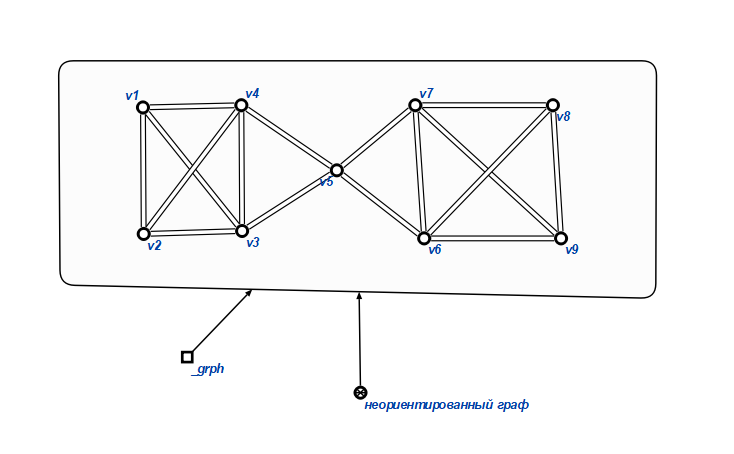
\includegraphics[width=0.45\textwidth, keepaspectratio]{fig/1.png}
\end{center}
\vspace{0.5pt}
\scriptsize Figure 12. The asymmetrical reconvergent integration of deterministic
knowledge processing operation as non-deterministic one (green lines)
with the divergent integration of deterministic knowledge processing
operation as deterministic operation one (red lines).

\begin{center}
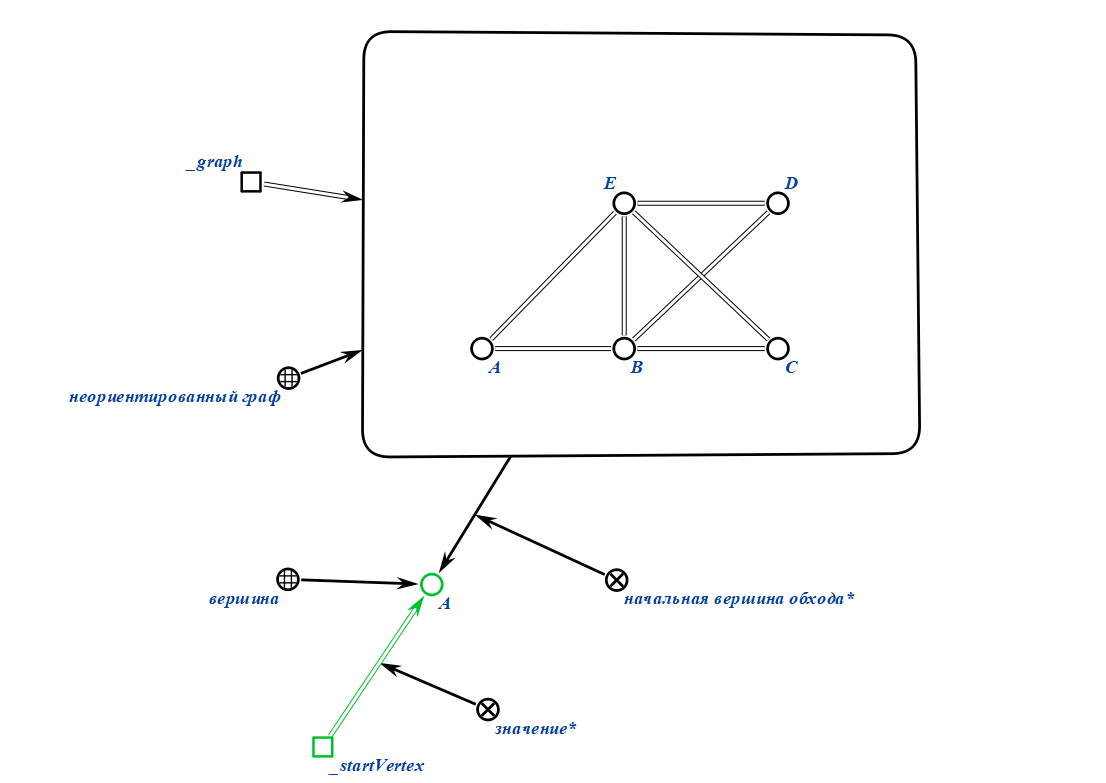
\includegraphics[width=0.45\textwidth, keepaspectratio]{fig/2.png}
\end{center}
\vspace{0.5pt}
\scriptsize Figure 13. The asymmetrical reconvergent integration of deterministic
knowledge processing operation as non-deterministic one (yellow
(diagonal) and green lines) with the asymmetrical divergent integration
of deterministic knowledge processing operation as non-deterministic
operation one (yellow (diagonal) and red lines).

\begin{center}
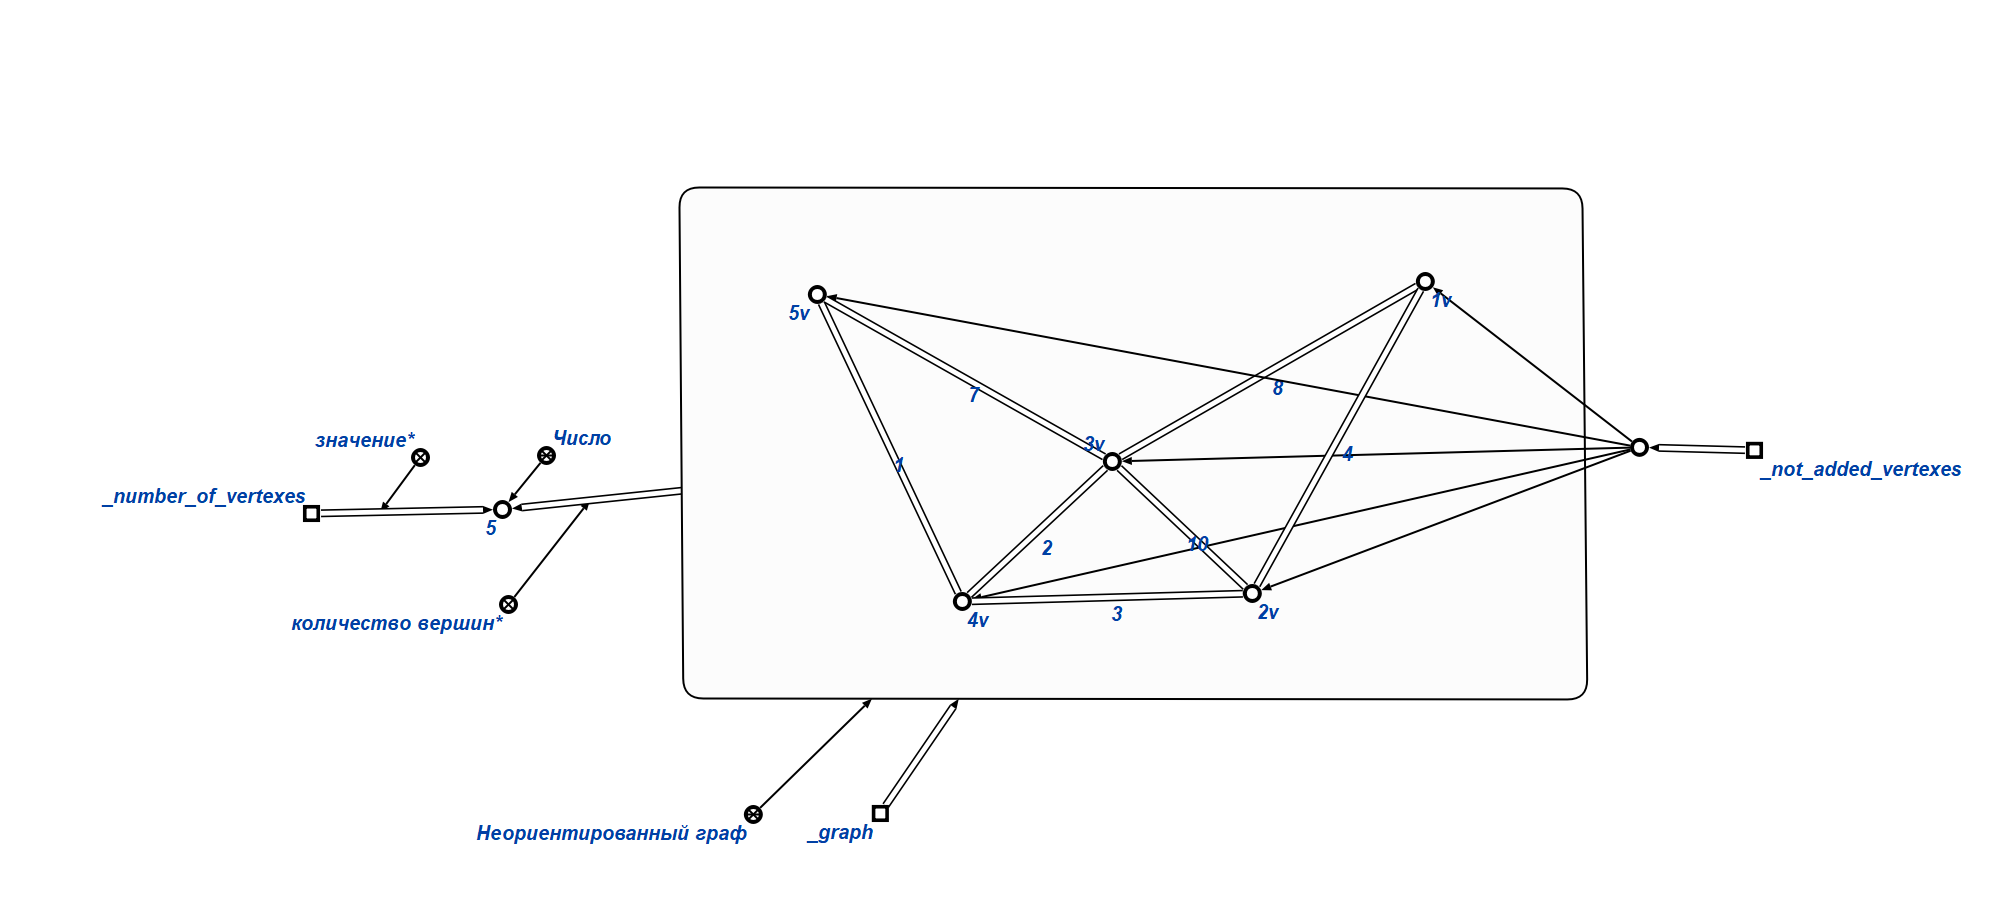
\includegraphics[width=0.45\textwidth, keepaspectratio]{fig/3.png}
\end{center}
\vspace{0.5pt}
\scriptsize Figure 14. The (symmetrical) reconvergent integration of deterministic
knowledge processing operation as non-deterministic one (yellow and
green lines) with the asymmetrical divergent integration of deterministic
knowledge processing operation as non-deterministic operation one
(yellow and red lines).


\begin{center}
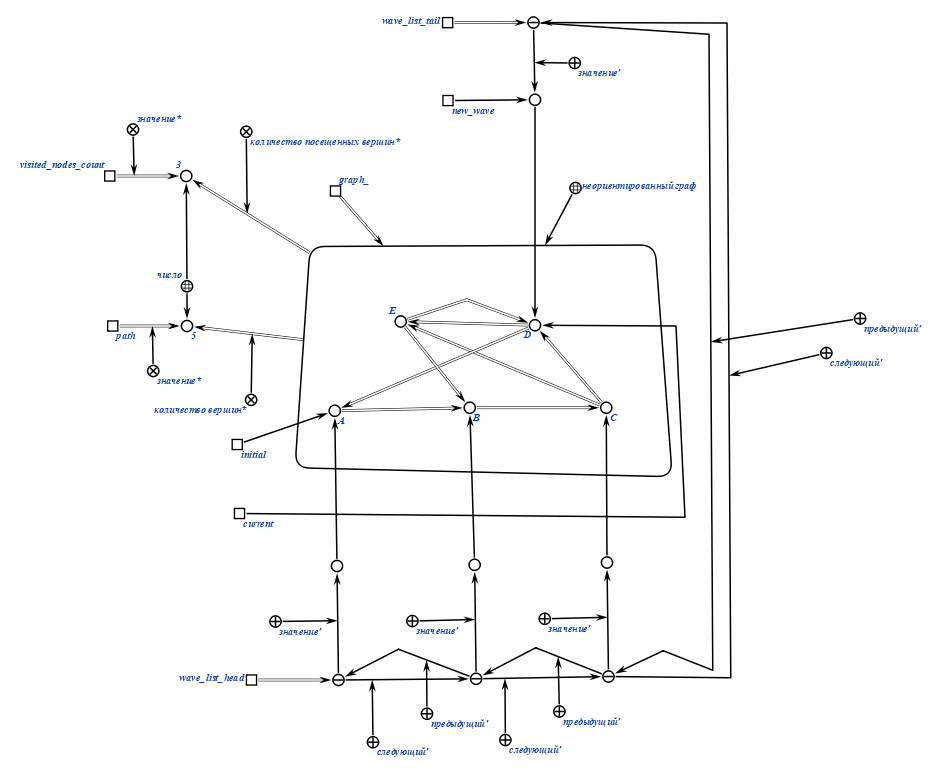
\includegraphics[width=0.45\textwidth, keepaspectratio]{fig/4.png}
\end{center}
\vspace{0.5pt}
\scriptsize Figure 15. The (symmetrical) reconvergent integration of deterministic
knowledge processing operation as non-deterministic one (yellow and
green lines) with the (symmetrical) divergent integration of deterministic
knowledge processing operation as non-deterministic operation one
(yellow and red lines).


\begin{center}
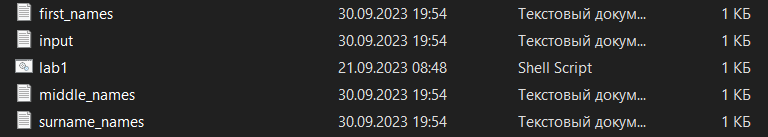
\includegraphics[width=0.45\textwidth, keepaspectratio]{fig/5.png}
\end{center}
\vspace{0.5pt}
\scriptsize Figure 16. The (symmetrical) reconvergent integration of deterministic
knowledge processing operation as non-deterministic one (green lines)
with the asymmetrical divergent integration of deterministic knowledge
processing operation as non-deterministic operation one (red lines).

\begin{center}
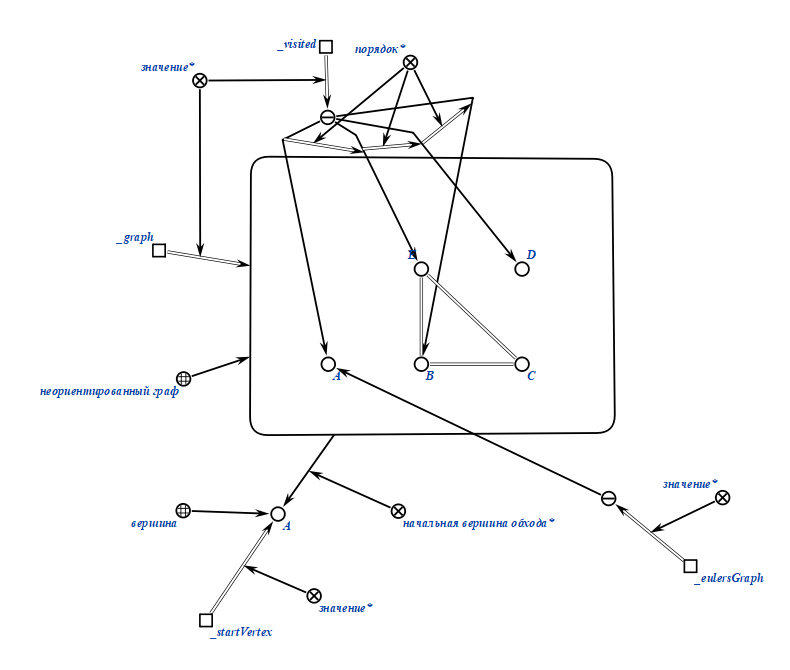
\includegraphics[width=0.45\textwidth, keepaspectratio]{fig/6.png}
\end{center}
\vspace{0.5pt}
\scriptsize Figure 17. The (symmetrical) reconvergent integration of deterministic
knowledge processing operation as non-deterministic one (green lines)
with the (symmetrical) divergent integration of deterministic knowledge
processing operation as deterministic operation one (red lines).

\begin{center}
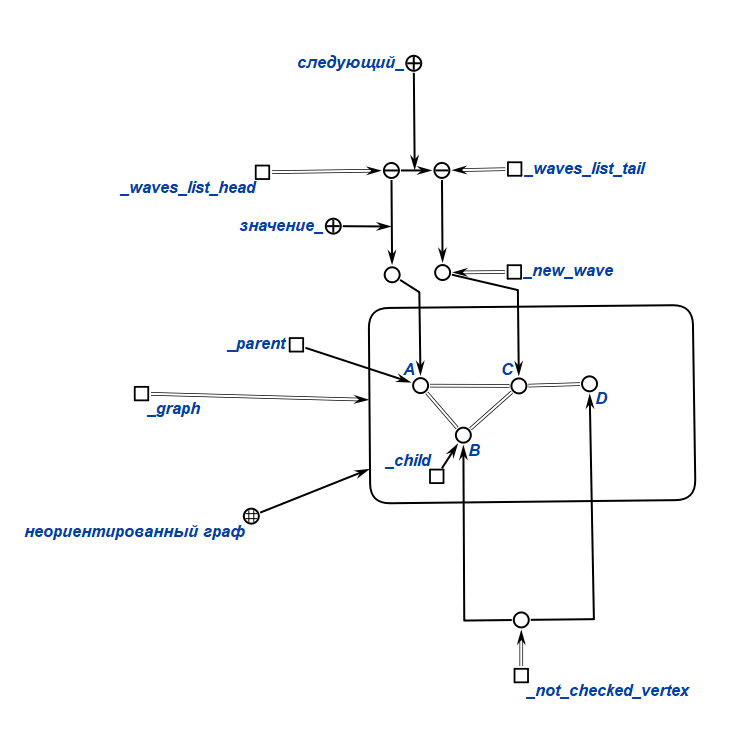
\includegraphics[width=0.45\textwidth, keepaspectratio]{fig/7.png}
\end{center}
\vspace{0.5pt}
\scriptsize Figure 18. The asymmetrical reconvergent integration of deterministic
knowledge processing operation as non-deterministic one (green lines)
with the asymmetrical divergent integration of deterministic knowledge
processing operation as non-deterministic operation one (red lines).

\begin{center}
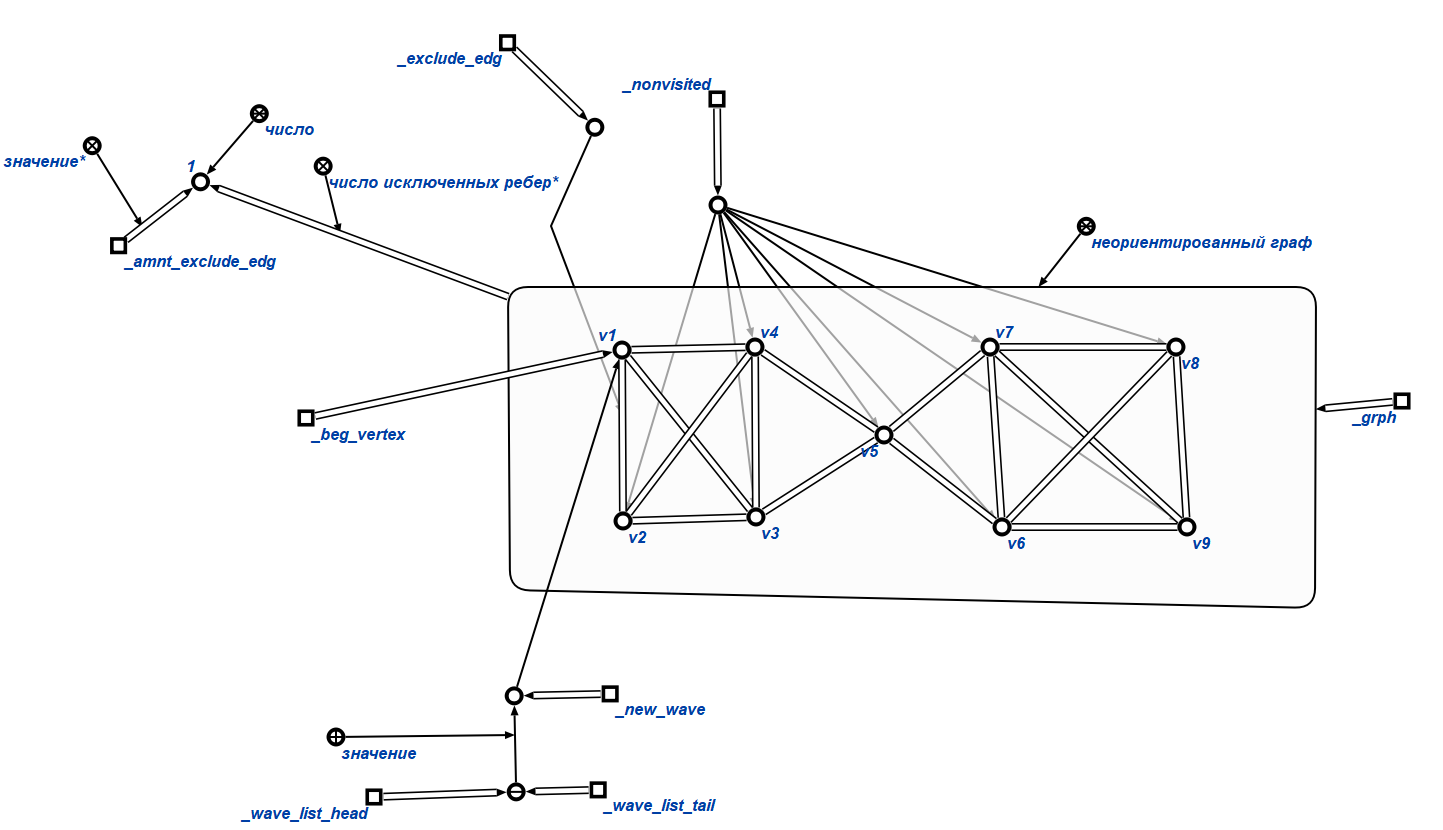
\includegraphics[width=0.45\textwidth, keepaspectratio]{fig/8.png}
\end{center}
\vspace{0.5pt}
\scriptsize Figure 19. The asymmetrical reconvergent integration of deterministic
knowledge processing operation as non-deterministic one (green lines)
with the (symmetrical) divergent integration of deterministic knowledge
processing operation as non-deterministic operation one (red lines).

\begin{center}
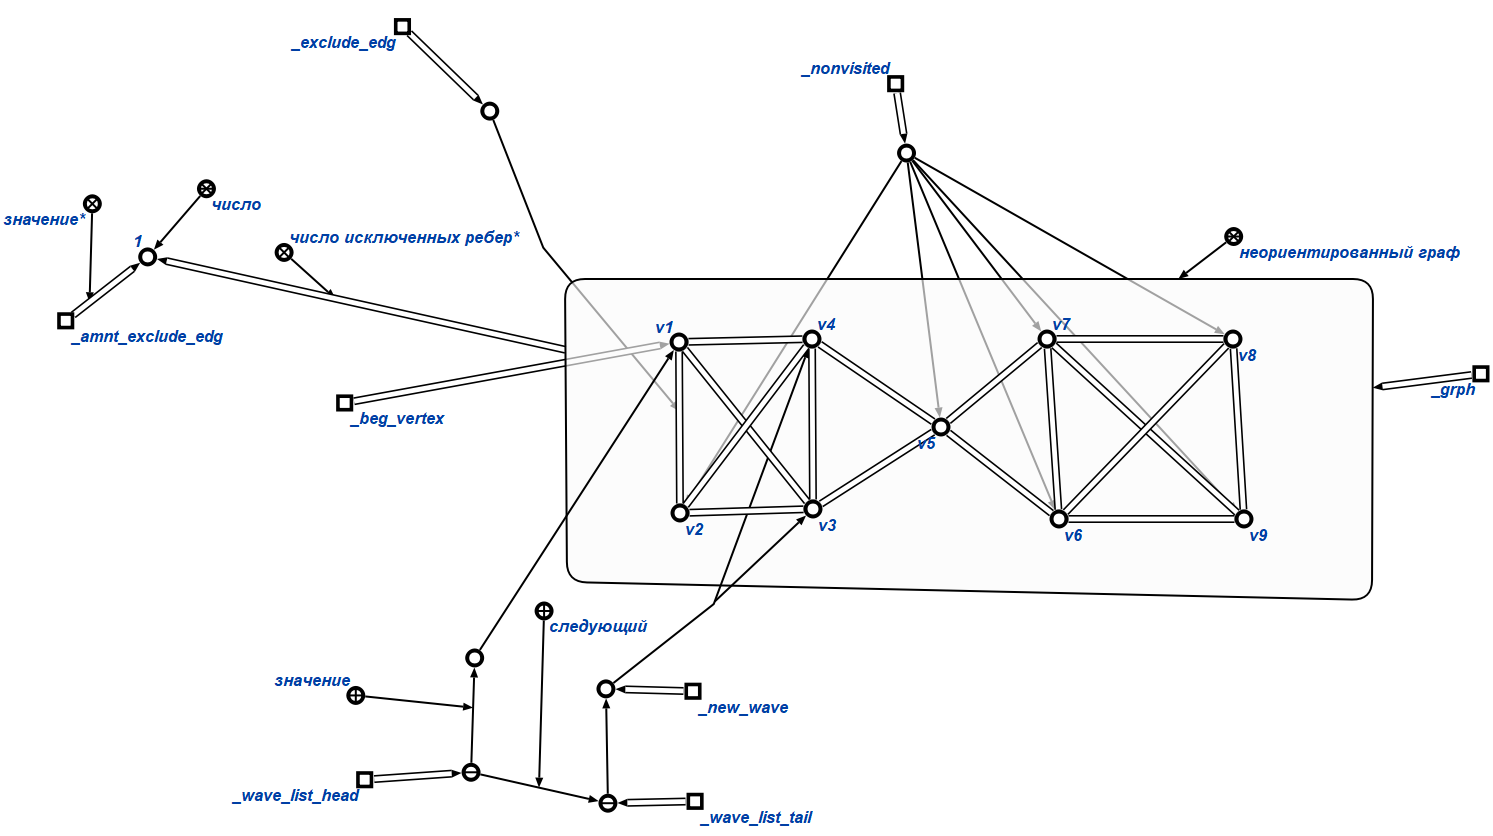
\includegraphics[width=0.45\textwidth, keepaspectratio]{fig/9.png}
\end{center}
\vspace{0.5pt}
\scriptsize Figure 20. The (symmetrical) reconvergent integration of deterministic
knowledge processing operation as deterministic one (green lines) with
the (symmetrical) divergent integration of deterministic knowledge
processing operation as non-deterministic operation one (red lines).


\begin{center}
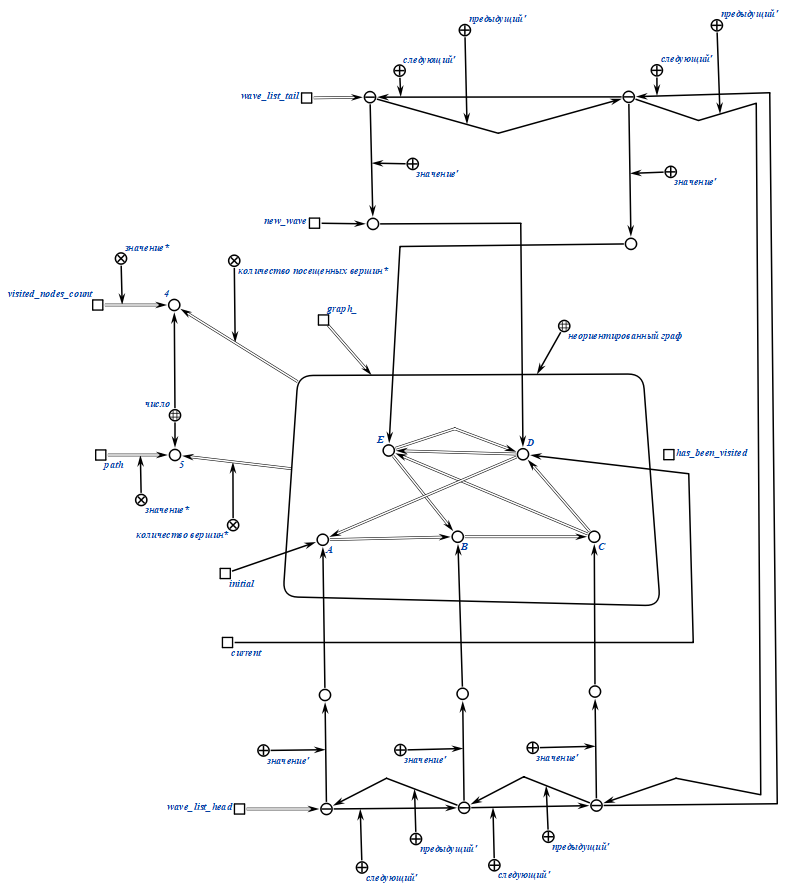
\includegraphics[width=0.45\textwidth, keepaspectratio]{fig/10.png}
\end{center}
\vspace{0.5pt}
\scriptsize Figure 21. The asymmetrical reconvergent integration of deterministic
knowledge processing operation as non-deterministic one (green lines)
with the asymmetrical divergent integration of deterministic knowledge
processing operation as non-deterministic operation one (red lines).



\begin{center}
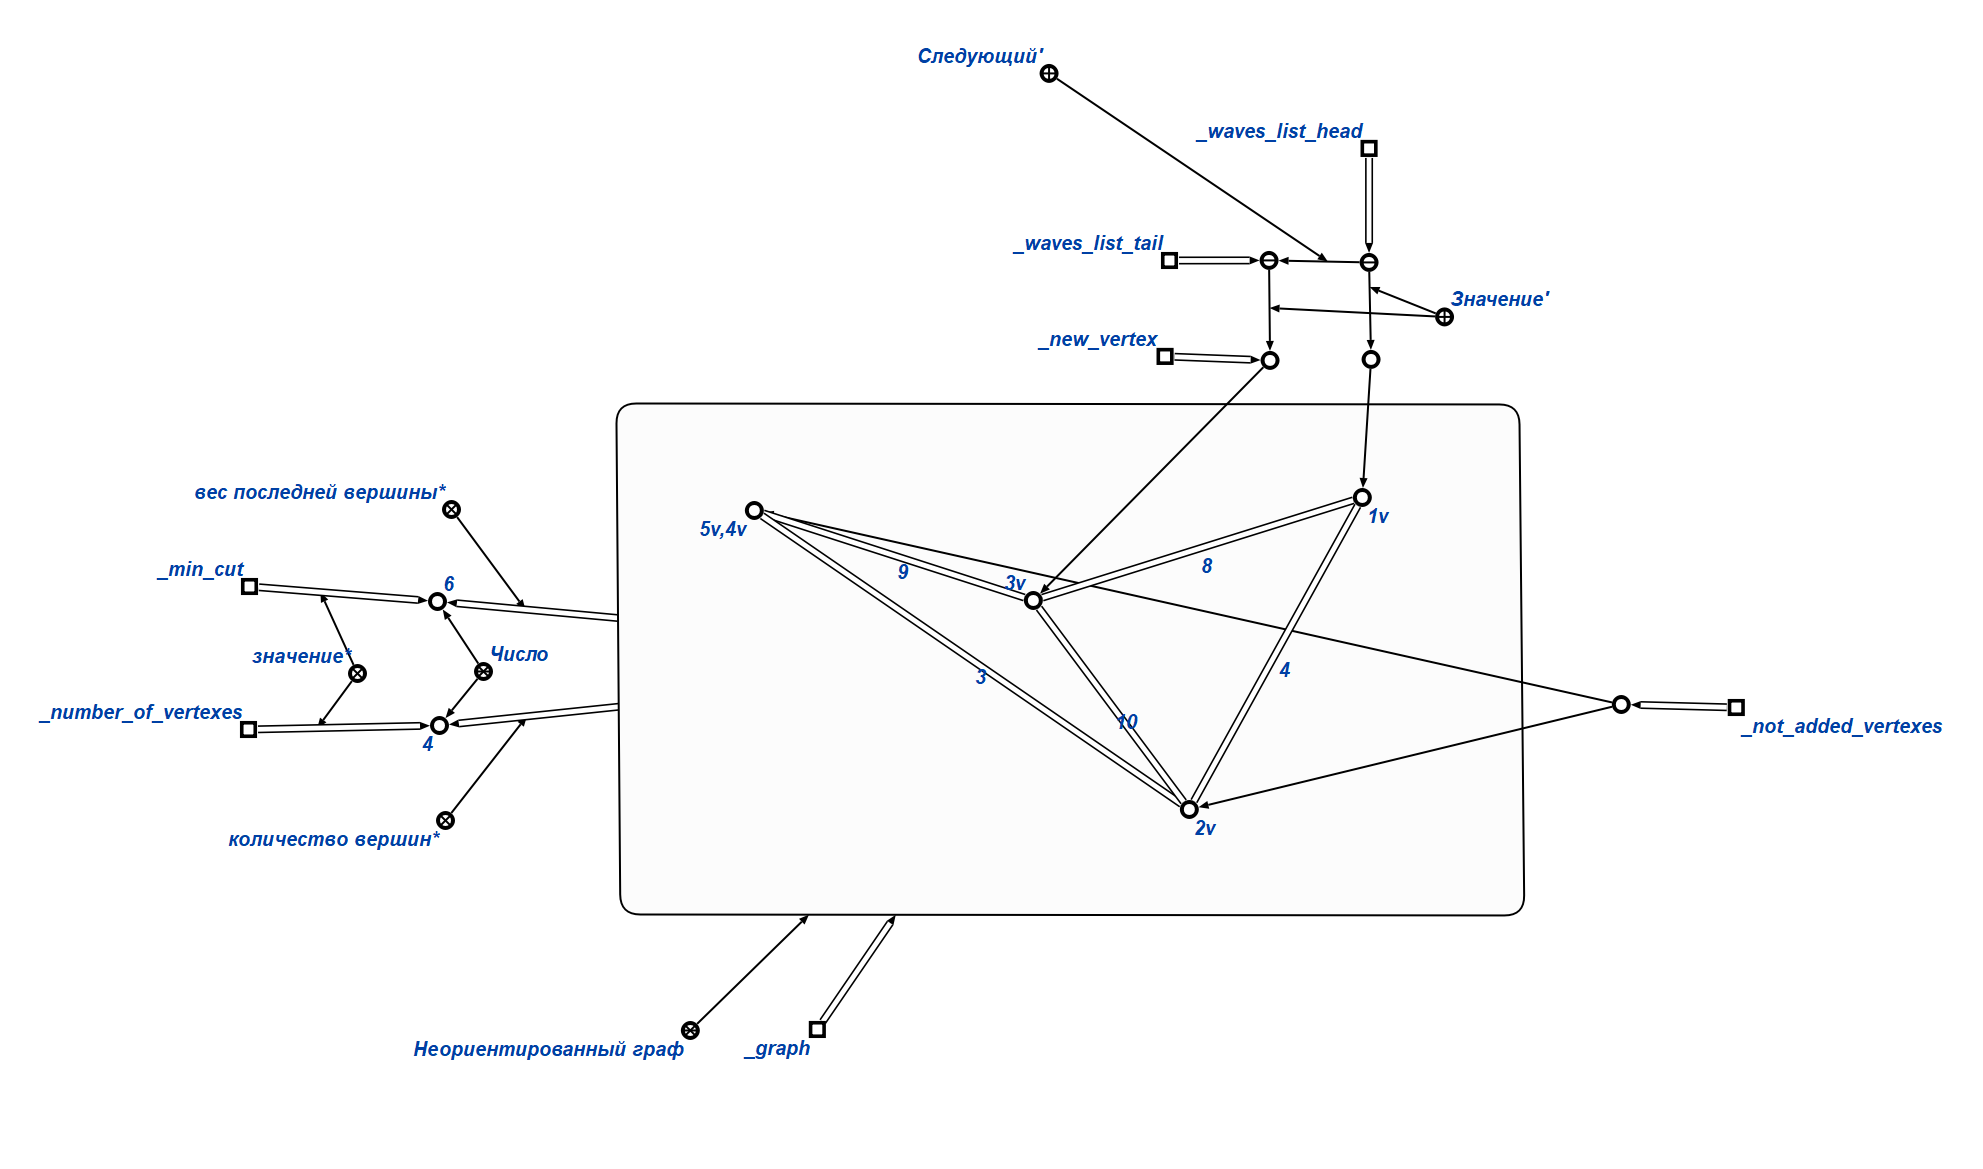
\includegraphics[width=0.45\textwidth, keepaspectratio]{fig/11.png}
\end{center}
\vspace{0.5pt}
\scriptsize Figure 22. The asymmetrical reconvergent integration of deterministic
knowledge processing operation as non-deterministic one (green lines)
with the asymmetrical divergent integration of deterministic knowledge
processing operation as non-deterministic operation one (red lines).


\begin{center}
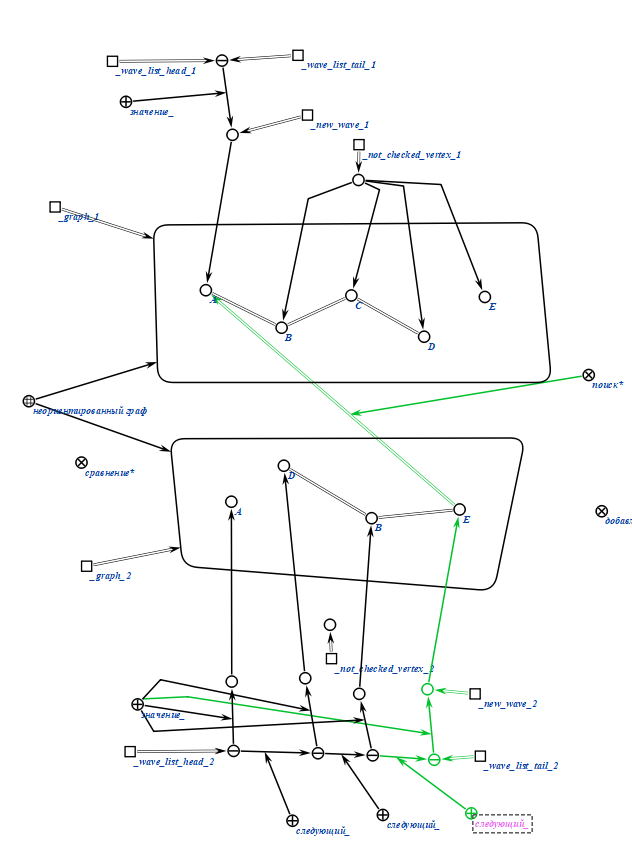
\includegraphics[width=0.45\textwidth, keepaspectratio]{fig/12.png}
\end{center}
\vspace{0.5pt}
\scriptsize Figure 23. The (symmetrical) reconvergent integration of deterministic
knowledge processing operation as deterministic one (green lines)
with the asymmetrical divergent integration of deterministic knowledge
processing operation as non-deterministic operation one (red lines).

\begin{center}
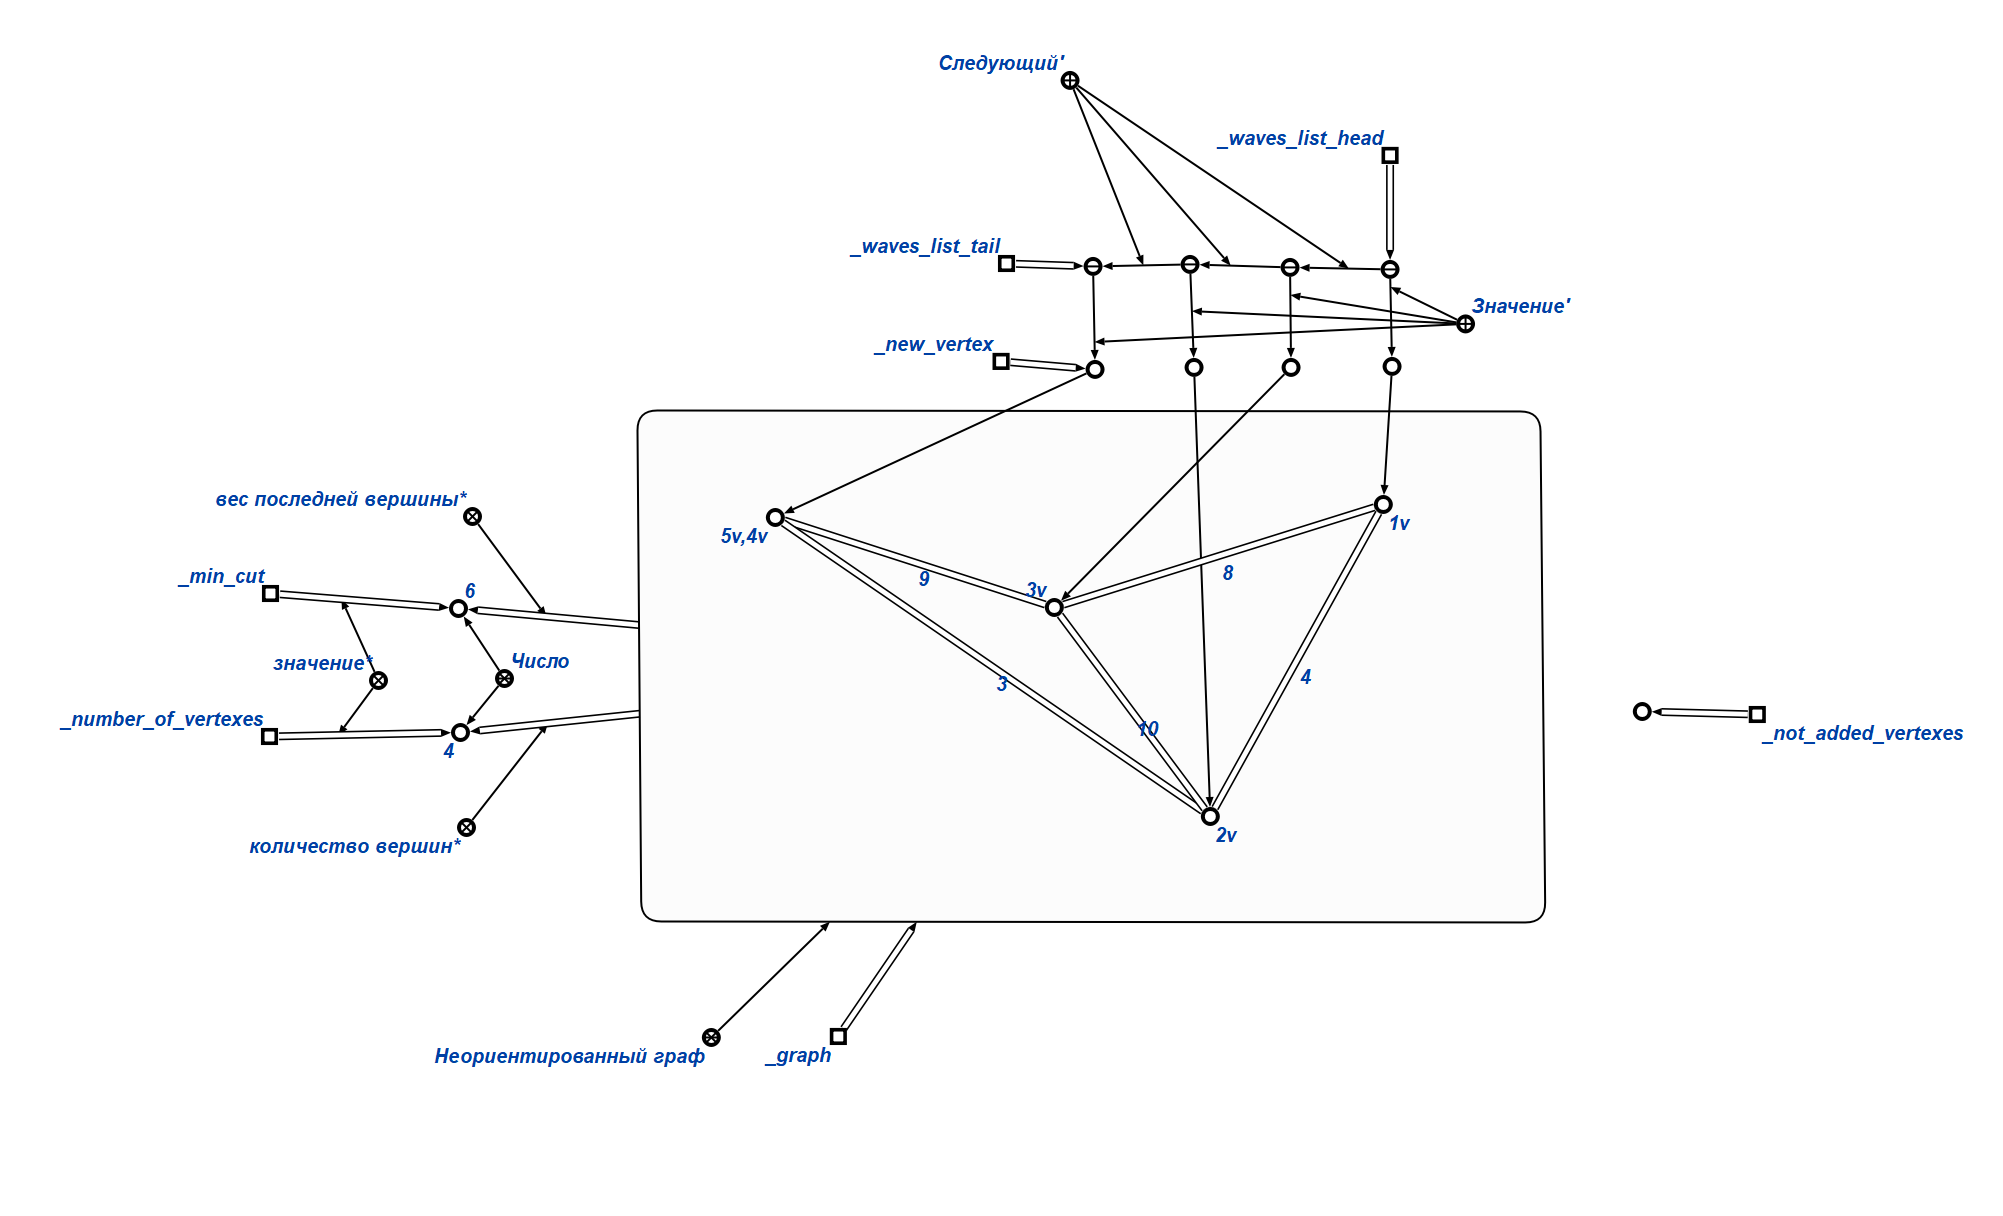
\includegraphics[width=0.45\textwidth, keepaspectratio]{fig/13.png}
\end{center}
\vspace{0.5pt}
\scriptsize Figure 24. The asymmetrical reconvergent integration of deterministic
knowledge processing operation as non-deterministic one (green lines)
with the (symmetrical) divergent integration of deterministic knowledge
processing operation as deterministic operation one (red lines).


\begin{center}
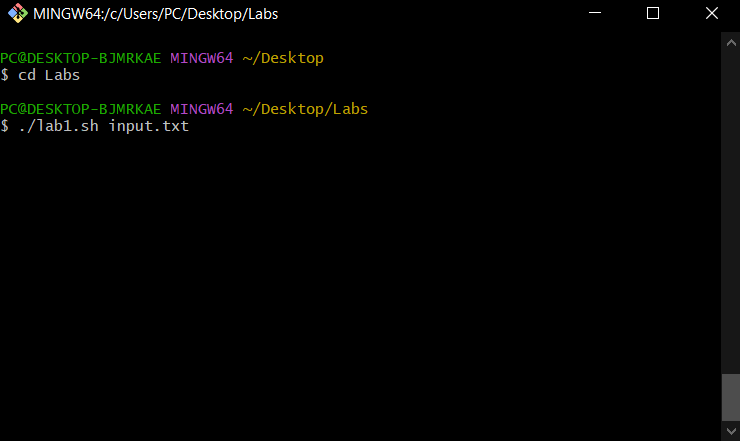
\includegraphics[width=0.45\textwidth, keepaspectratio]{fig/14.png}
\end{center}
\vspace{0.5pt}
\scriptsize Figure 25. The (symmetrical) reconvergent integration of deterministic
knowledge processing operation as non-deterministic one (green lines)
with the asymmetrical divergent integration of deterministic knowledge
processing operation as non-deterministic operation one (red lines).

\normalsize

states (sets of formulas), and in the second case, they are
formulas.

\vspace{10pt}
 
\centerline{\{($A \rightarrow B$),($B \rightarrow C$) $\vdash$ ($A \rightarrow B$),($B \rightarrow C$),($A \rightarrow C$)\}}
\centerline{\{($D \rightarrow B$),($B \rightarrow E$) $\vdash$ ($D \rightarrow B$),($B \rightarrow E$),($D \rightarrow E$)\}} 
\centerline{\{($A \rightarrow B$),($B \rightarrow C$) $\cup$ ($D \rightarrow B$),($B \rightarrow E$)\}} 
\centerline{\{($A \rightarrow B$),($B \rightarrow C$),($A \rightarrow C$),($D \rightarrow C$),} 
\centerline{($D \rightarrow B$),($B \rightarrow E$),($D \rightarrow E$),($A \rightarrow E$)\}}

\hspace{0.27cm}For classical logics and logical models of knowledge
processing, it is possible to naturally introduce a metric
on sets of literal conjuncts (of a given length), if we take
a finite subject domain and accept the assumption (hypothesis) of a closed world, then the metric is introduced
as the sum of exclusive-OR from each pairs of matching
literals.
\vspace{10pt}

\centerline{$\mu(⟨x, y⟩) = \sum\limits_{i=1}^{n} x_i \vee y_i$}

\vspace{10pt}
Moreover, if the conjuncts define a set-ring algebra, then
we can speak of a normed space and a norm (valuation)
over a vector space, where the field is GF(2). Any
(meaningful) proposition over this domain, except for
the identically false one, can be represented as (PDNF).
Then for PDNF we get a metric vector. The proposition
is true if and only if the metric vector contains 0. For
PCNF, there is no 0.

\vspace{10pt}

\centerline{$\mu(⟨x, y⟩) = min_j\sum\limits_{i=1}^{n} x_ij \vee y_ij$}

\vspace{10pt}

\hspace{0.27cm}In addition to (null-local predicates) of literals (constants), unary (semantic) predicates for the type of an
element of an sc-text and unary and binary (syntactic)
predicates for element incidence tuples (variables) can
be considered (by analogy of relation algebra [22], [23]).
In the case of search by pattern (homomorphism), the
metric is calculated on multisets. Possible task is to
minimize (maximize) the metric from the pragmatic
view of logics. Associated with the search for a relevant
structure, this task is of practical importance in reference
and testing (checking) (dialog) systems [21], [24]. Also,
metrics with other quantor elimination approaches ( [23],
[25]) can be used for logical inference and theorem
proving purposes. The system of natural inference and
sequent calculus consider finite sets of formulas. One
of the algorithms for solving inference problems is
a conflict-driven (contradiction-driven) clause learning
(CDCL) [26]. These techniques seemed to be promising.
To express complex patterns and regularities, it is possible
to construct a metatheory using metastructures. For this,
meta-relations and modal operators are introduced. Such
a formalism allows describing the complex introspective
reasoning characteristic of modal logics (see Fig. 26–28
for the sages hat puzzle solution [27]).
\hspace{0.27cm}Applied logics [27]–[32] consider applications of
classical logic to abstract and subject domains describing
reality: logical theories about equality and order relations
[28], [29], logical theories of arithmetic [28], logical
theories of time [27], [31], logical proof theories [28],
[30], graph and geometric theories [32], theories of natural
and social systems [29].
\hspace{0.27cm}Classification of logical theories corresponds to the
classification of subject domains. Let us consider some
concepts and examples that are considered within applied
logics.

\vspace{10pt} 

\begin{tabbing}
 \textbf{\textit{slot binary relation}} \\ $\Rightarrow$ \hspace{0.5cm} \= \textit{note}*: \\ \>[slot binary relation is a slot sc-relation that is a  \\ \> 
set.]
\end{tabbing}

\begin{tabbing}
 \textbf{\textit{non-slot binary relation}} \\ $\Rightarrow$ \hspace{0.5cm} \= \textit{note}*: \\ \>[non-slot binary relation is a binary sc-relation \\ \> 
that is a set but is not a slot sc-relation.]]
\end{tabbing}

\begin{tabbing}
 \textbf{\textit{irreflexive slot binary relation}} \\ $\subset$ \hspace{0.5cm} \= \textit{irreflexive binary relation}
 \\ $\Rightarrow$ \hspace{0.5cm} \= 

 \textit{note}*: 
\end{tabbing}



\end{multicols}
\end{document}
